\documentclass[12pt, a4paper, oneside]{article}\usepackage[]{graphicx}\usepackage[]{color}
%% maxwidth is the original width if it is less than linewidth
%% otherwise use linewidth (to make sure the graphics do not exceed the margin)
\makeatletter
\def\maxwidth{ %
  \ifdim\Gin@nat@width>\linewidth
    \linewidth
  \else
    \Gin@nat@width
  \fi
}
\makeatother

\definecolor{fgcolor}{rgb}{0.345, 0.345, 0.345}
\newcommand{\hlnum}[1]{\textcolor[rgb]{0.686,0.059,0.569}{#1}}%
\newcommand{\hlstr}[1]{\textcolor[rgb]{0.192,0.494,0.8}{#1}}%
\newcommand{\hlcom}[1]{\textcolor[rgb]{0.678,0.584,0.686}{\textit{#1}}}%
\newcommand{\hlopt}[1]{\textcolor[rgb]{0,0,0}{#1}}%
\newcommand{\hlstd}[1]{\textcolor[rgb]{0.345,0.345,0.345}{#1}}%
\newcommand{\hlkwa}[1]{\textcolor[rgb]{0.161,0.373,0.58}{\textbf{#1}}}%
\newcommand{\hlkwb}[1]{\textcolor[rgb]{0.69,0.353,0.396}{#1}}%
\newcommand{\hlkwc}[1]{\textcolor[rgb]{0.333,0.667,0.333}{#1}}%
\newcommand{\hlkwd}[1]{\textcolor[rgb]{0.737,0.353,0.396}{\textbf{#1}}}%

\usepackage{framed}
\makeatletter
\newenvironment{kframe}{%
 \def\at@end@of@kframe{}%
 \ifinner\ifhmode%
  \def\at@end@of@kframe{\end{minipage}}%
  \begin{minipage}{\columnwidth}%
 \fi\fi%
 \def\FrameCommand##1{\hskip\@totalleftmargin \hskip-\fboxsep
 \colorbox{shadecolor}{##1}\hskip-\fboxsep
     % There is no \\@totalrightmargin, so:
     \hskip-\linewidth \hskip-\@totalleftmargin \hskip\columnwidth}%
 \MakeFramed {\advance\hsize-\width
   \@totalleftmargin\z@ \linewidth\hsize
   \@setminipage}}%
 {\par\unskip\endMakeFramed%
 \at@end@of@kframe}
\makeatother

\definecolor{shadecolor}{rgb}{.97, .97, .97}
\definecolor{messagecolor}{rgb}{0, 0, 0}
\definecolor{warningcolor}{rgb}{1, 0, 1}
\definecolor{errorcolor}{rgb}{1, 0, 0}
\newenvironment{knitrout}{}{} % an empty environment to be redefined in TeX

\usepackage{alltt} % Paper size, default font size and one-sided paper
%\graphicspath{{./Figures/}} % Specifies the directory where pictures are stored
%\usepackage[dcucite]{harvard}
%\usepackage{rotating}
\usepackage{amsmath}
%\usepackage{setspace}
\usepackage{pdflscape}
\usepackage[flushleft]{threeparttable}
%\usepackage{multirow}
\usepackage[comma, sort&compress]{natbib}% Use the natbib reference package - read up on this to edit the reference style; if you want text (e.g. Smith et al., 2012) for the in-text references (instead of numbers), remove 'numbers' 
\usepackage{graphicx}
%\bibliographystyle{plainnat}
\bibliographystyle{agsm}
\usepackage[colorlinks = true, citecolor = blue, linkcolor = blue]{hyperref}
%\hypersetup{urlcolor=blue, colorlinks=true} % Colors hyperlinks in blue - change to black if annoying
%\renewcommand[\harvardurl]{URL: \url}
\IfFileExists{upquote.sty}{\usepackage{upquote}}{}
\begin{document}
\title{Introduction to Time Series Analysis}
\author{Rob Hayward}
\date{\today}
\maketitle
%\begin{abstract}
%erehrere
%\end{abstract}


\section{ARMA(p,q) time series}
This comes from \href{http://freakonometrics.hypotheses.org/12217}{Arthur Charptentier}.  Given the ARMA(1,1) model
\begin{equation}
X_t = \phi X_{t-1} + \varepsilon_t + \theta \varepsilon_{t-1}
\end{equation}

\begin{knitrout}
\definecolor{shadecolor}{rgb}{0.969, 0.969, 0.969}\color{fgcolor}\begin{kframe}
\begin{alltt}
theta = 0.7
phi = 0.5
n = 1000
Z = \hlkwd{rep}(0, n)
\hlkwd{set.seed}(1)
e = \hlkwd{rnorm}(n)
\hlkwd{for} (t in 2:n) Z[t] = phi * Z[t - 1] + e[t] + theta * e[t - 1]
Z = Z[800:1000]
\hlkwd{plot}(Z, type = \hlstr{"l"}, main = \hlstr{"\hlkwd{ARMA}(1,1) process"})
\end{alltt}
\end{kframe}
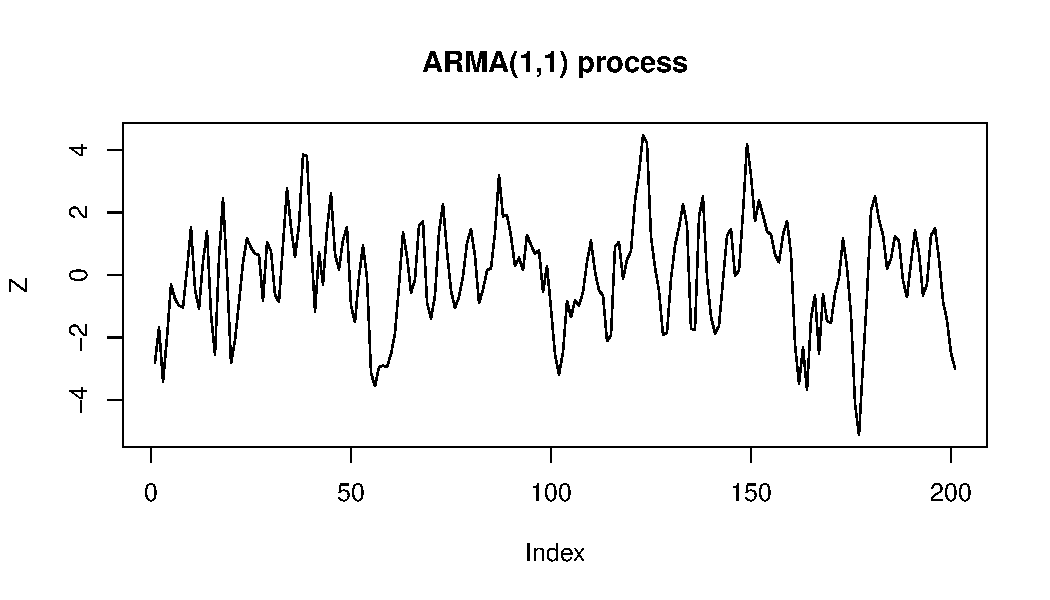
\includegraphics[width=\maxwidth]{figure/MA} 

\end{knitrout}

If the MA element is not identified and purely AR model is estimated by least squres the estimate of $\phi$ is not consistent. 
\begin{equation}
X_t = \phi X_{t-1} + \varepsilon_t
\end{equation}

\begin{knitrout}
\definecolor{shadecolor}{rgb}{0.969, 0.969, 0.969}\color{fgcolor}\begin{kframe}
\begin{alltt}
base = \hlkwd{data.frame}(Y = Z[2:n], X = Z[1:(n - 1)])
regression = \hlkwd{lm}(Y ~ 0 + X, data = base)
\hlkwd{summary}(regression)
\end{alltt}
\begin{verbatim}
## 
## Call:
## lm(formula = Y ~ 0 + X, data = base)
## 
## Residuals:
##    Min     1Q Median     3Q    Max 
## -3.245 -0.791  0.063  0.971  3.069 
## 
## Coefficients:
##   Estimate Std. Error t value Pr(>|t|)    
## X    0.696      0.051    13.6   <2e-16 ***
## ---
## Signif. codes:  0 '***' 0.001 '**' 0.01 '*' 0.05 '.' 0.1 ' ' 1 
## 
## Residual standard error: 1.22 on 199 degrees of freedom
##   (799 observations deleted due to missingness)
## Multiple R-squared: 0.483,	Adjusted R-squared: 0.481 
## F-statistic:  186 on 1 and 199 DF,  p-value: <2e-16
\end{verbatim}
\end{kframe}
\end{knitrout}

Compute the autocorreltion of the noise.  
\begin{knitrout}
\definecolor{shadecolor}{rgb}{0.969, 0.969, 0.969}\color{fgcolor}\begin{kframe}
\begin{alltt}
n = 200
\hlkwd{cor}(\hlkwd{residuals}(regression)[2:n], \hlkwd{residuals}(regression)[1:(n - 1)])
\end{alltt}
\begin{verbatim}
## [1] 0.2663
\end{verbatim}
\end{kframe}
\end{knitrout}

More formlly, with the Durbin-Watson sttistic
\begin{knitrout}
\definecolor{shadecolor}{rgb}{0.969, 0.969, 0.969}\color{fgcolor}\begin{kframe}
\begin{alltt}
\hlkwd{require}(car)
\end{alltt}


{\ttfamily\noindent\itshape\color{messagecolor}{\#\# Loading required package: car}}\begin{alltt}
\hlkwd{durbinWatsonTest}(regression)
\end{alltt}
\begin{verbatim}
##  lag Autocorrelation D-W Statistic p-value
##    1          0.2657         1.463   0.002
##  Alternative hypothesis: rho != 0
\end{verbatim}
\end{kframe}
\end{knitrout}

It should be assumed that 
\begin{equation}
u_t = \varepsilon_t + \theta \vrepsilon_{t-1}
\end{equation}
and 
\begin{equation}
\rho(1) = \frac{\theta}{1 + \theta^2}
\end{equation}
\begin{knitrout}
\definecolor{shadecolor}{rgb}{0.969, 0.969, 0.969}\color{fgcolor}\begin{kframe}
\begin{alltt}
\hlkwd{polyroot}(\hlkwd{c}(1, -1/\hlkwd{cor}(\hlkwd{residuals}(regression)[2:n], \hlkwd{residuals}(regression)[1:(n - 
    1)]), 1))
\end{alltt}
\begin{verbatim}
## [1] 0.2885-0i 3.4666+0i
\end{verbatim}
\end{kframe}
\end{knitrout}





\end{document}
